\section[Biological traits]{Biological traits of phytoplankton}
\subsection{A difficult definition}
Despite being the definition of the subject the first thing to be done in a thesis work, talking about plankton can be somehow vague. Take as an example the definition given in \autocite[chapter 1.1, pag. 2]{reynolds2006ecology}\footnote{The etymology of the name comes from the Greek \textgreek{πλαγκτός}, ``planktòs'', describing a wandering object.}: 
\begin{quotation}
living seston [i.e. not-soluted matter], adapted for a life spent wholly or partly in quasi-suspension in open water, and whose powers of motility do not exceed turbulent entrainment
\end{quotation}
which necessarily includes a variety of organisms, ranging from unicellular ones to small multicellular animals (e.g. members from the phylum Cnidaria, like ctenophores) and not taking into account their biological and trophic role. The paraphyletic character of this definition is useful
\footnote{A grouping of species is said to be paraphiletic if it excludes at least one descendant of an ancestor \autocite[pag. 4]{wiley2015compleat}}:
a passively moving being experiences a different environment from what an active swimmer does, and considering all this passive organisms together is in some ways natural. However, there is not such a sharp distinction, as one can see considering the example of a jellyfish, which is with no doubt an active swimmer, but is clearly carried from currents; a way to give sense to this definition is then to refer it to \textit{small scale} motion, which plankton cannot oppose, whereas ``actively swimming'' creatures are transported by currents whose scale is bigger. A simpler way to state this is to say that plankton is passively transported by a current \autocite{Lalli1997}\\
Moreover, such a classification lacks any information about the ecological role of plankton: indeed, \textit{phytoplankton} (``plant-plankton'' from the Greek \textgreek{φυτόν}, ``phytòn'') and \textit{zooplankton} (``animal-plankton'' from \textgreek{ζῴον}, ``zòon'') are two categories which discriminate, respectively, from autotrophic and eterotrophic organisms (see \autoref{sec:mixotrophy}. Zooplanktonic species are capable of swimming, and are usually bigger than phytoplanktonic ones: unicellular organisms (flagellates, Foraminifera, Radiolaria, ciliates), jellyfishes, ctenophores, small crustaceans (copepods), fish larvae (``ichthyoplankton'', ``fish-plankton'', from \textgreek{ἰχθύς}, ``ikhthys'') are included in this category\autocite[chapter 4]{Lalli1997}. Phytoplanktonic species, which are mainly dinoflagellates and diatoms (often creating filaments or other aggregates, with the aid of spines or mucilaginous matter), are generally unicellular organisms and are the feeding source of zooplankton; the term ``grazing'' refers to this behaviour. Phytoplanktic species are somehow uniform in their charasterictics, a trait which Reynolds refers to as the result of convergent evolution \autocite[chapter 1.4]{reynolds2006ecology}. Nevertheless, they can assume many shapes and their dimension varies in the range $10^{-7}\div10^{-2}m$.

\subsubsection{Mixotrophy} \label{sec:mixotrophy}
Moreover, making it more difficult to classify plankton, \textit{mixotrophy}, or the condition of coexistence of both photoautotrophy and phagoheterotrophy in the same organism, appears to be more common than it was believed. \textit{Photoautotrophy} (from \textgreek{φῶς}, ``fòs'', light;  \textgreek{αὐτός}, ``autós'', “self”;  \textgreek{τροφή}, ``trophé'', “nourishment”) refers to the ability of "fixate" carbon, i.e. acquiring it from inorganic compounds and converting it to organic ones, usable from organisms; \textit{phagoeterotrophy} (from \textgreek{φᾰγεῖν}, ``phagéin'', to eat); \textgreek{ἕτερος} ``héteros'', other) refers to the acquisition of carbon by predate it from other organisms. Mixotrophs result dominant in the most part of environments \autocite{Stoecker2009AcquiredProtists} and a classification has been proposed in \autocite{Mitra2016DefiningStrategies} which takes into account the fact that organisms can acquire photosyntetic capabilities from other microorganisms, either retaining the functional parts of them, or incorporating them as a whole. In the article, \textit{in silico} experiments are reported which confirm a dominance of mixotrophs over ``traditional'' strategies. 

\subsection{Blooms} \label{sec:ref_pla_blooms}
When the right conditions occur, phytoplankton colonies can form ``blooms'', that is extended areas with a high density of cells. A characteristic feature of this events is the high rate of growth \autocite{Taylor2011ShutdownBlooms}.\\
Although blooms are a natural phenomenon, useful to the environment since phytoplankton produces at least 50\% of the oxygen on the planet, their anomalous occurrence can be dangerous both to human and animal life. 
% FONTE OX
Apart of the aesthetic and touristic damage which such formations can provoke, Plankton blooms represent a serious issue both because their rapid growth requires oxygen, thus reducing its concentration (\textit{anoxic} conditions) and because many species produce toxins (saxitoxin, domoic acid): indeed, massive deaths of fishes and even marine mammals occur as a consequence of blooms \autocite[chapter 3]{Lalli1997}. \\
Blooms are observed both in marine water and in lakes. In the latter experiments have been done to influence the growth rates of cyanobacteria with an artificially induced mixing, with notable effects \autocite{Visser2016ArtificialReview}: the resulting rate of growth is suppressed out of an eutrophic, i.e. favourable to growth, interval.\\
Satellite images have proven useful to track the plankton in sea, where direct measures would be highly difficult. Some examples of these images are shown in \autoref{fig:sat_barent}, \autoref{fig:sat_finland}, \autoref{fig:sat_kamchatka}, where the close resemblance of the shape of the phytoplankton blooms to the flow of water is notable
%\footnote{ for \autoref{fig:sat_barent} and \autoref{fig:sat_finland}; \url{https://earthobservatory.nasa.gov/features/Phytoplankton/page2.php} for \autoref{fig:sat_kamchatka}.}. 
In \autoref{fig:sat_barent} and \autoref{fig:sat_finland}, shot in real colours, two different kind of blooms are visible: in the first image, the white colour is probably due to the ``coccolithophores, which have tiny, chalky, calcium carbonate shells'', while the second one shows cyanobacteria (a green colour could come from diatoms, too).
\footnote{\url{https://earthobservatory.nasa.gov/images/92462/summer-blooms-in-the-baltic-and-barents}}. 
In \autoref{fig:sat_kamchatka} the same image is shown both in true and in false colours, evidencing the chlorophyll concentration, which is one of the trackers commonly utilized for phytoplankton (see \autoref{sec:distribution}).

\begin{figure} [H]
    \centering
    \begin{subfigure}[b]{.45\textwidth}
        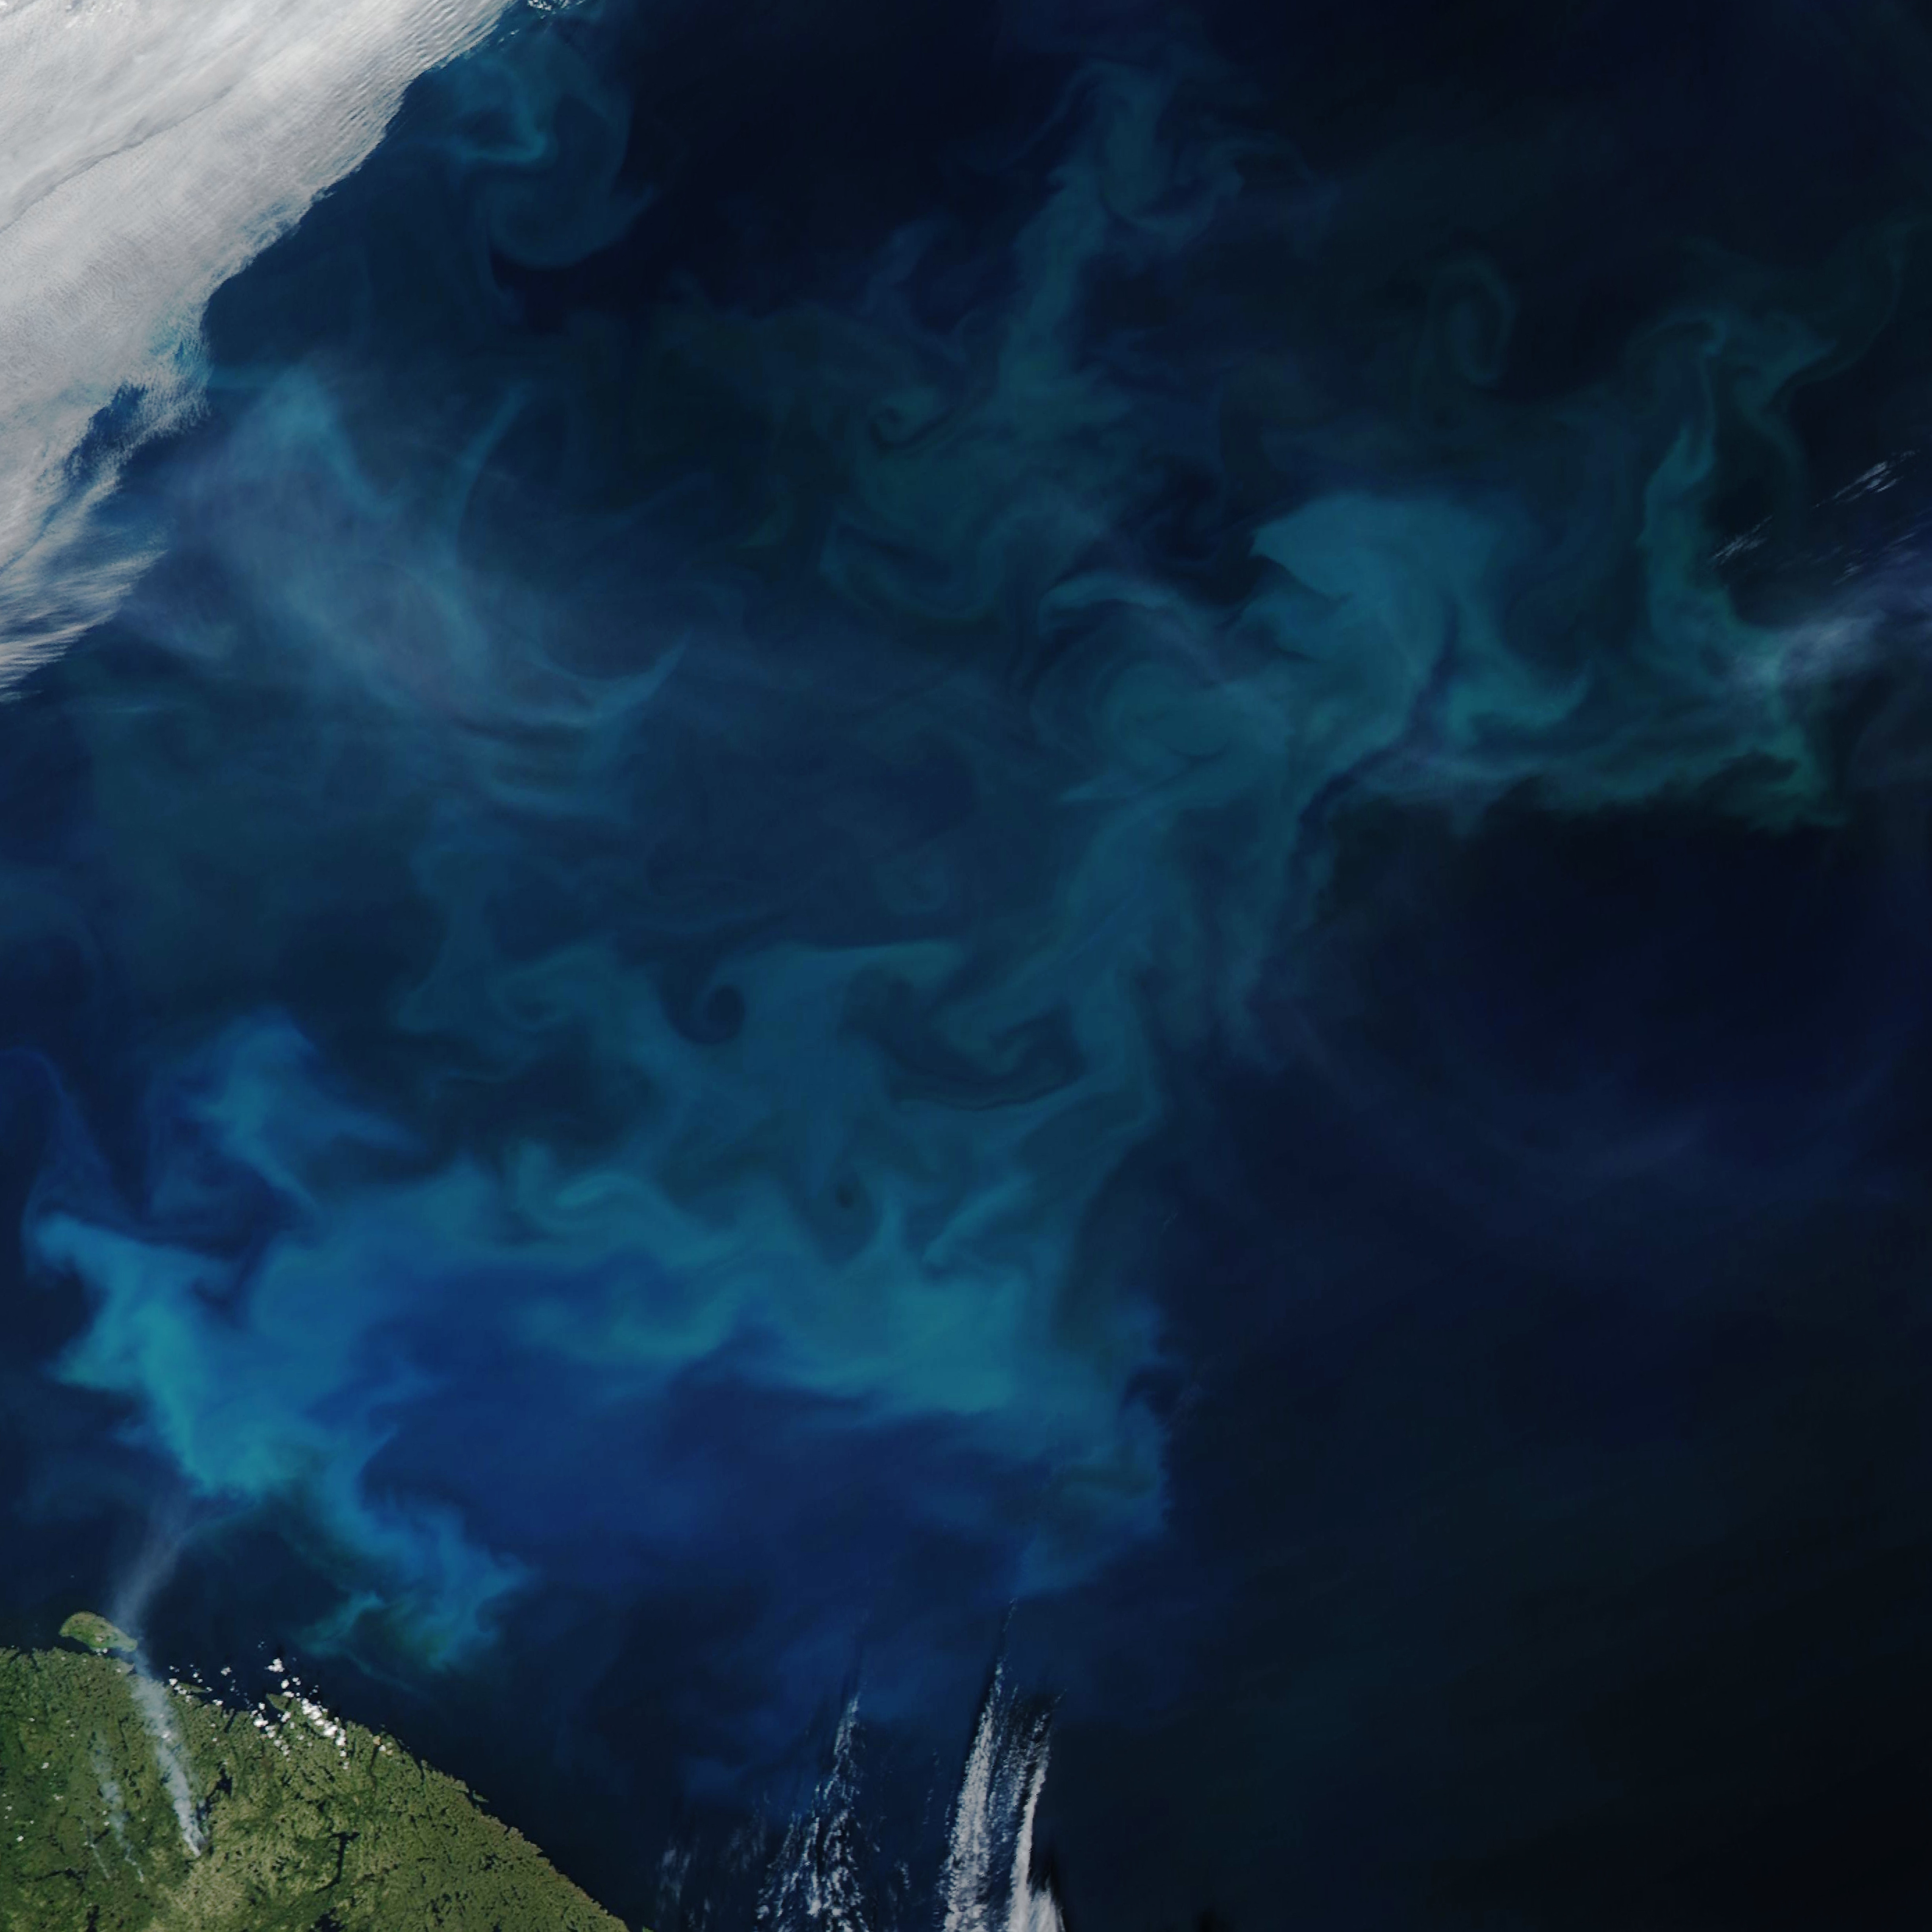
\includegraphics[height=\textwidth]{img/barentseabloom_amo_2018201_lrg.jpg}
        \caption{}
        \label{fig:sat_barent}
    \end{subfigure}
    \begin{subfigure}[b]{.45\textwidth}
        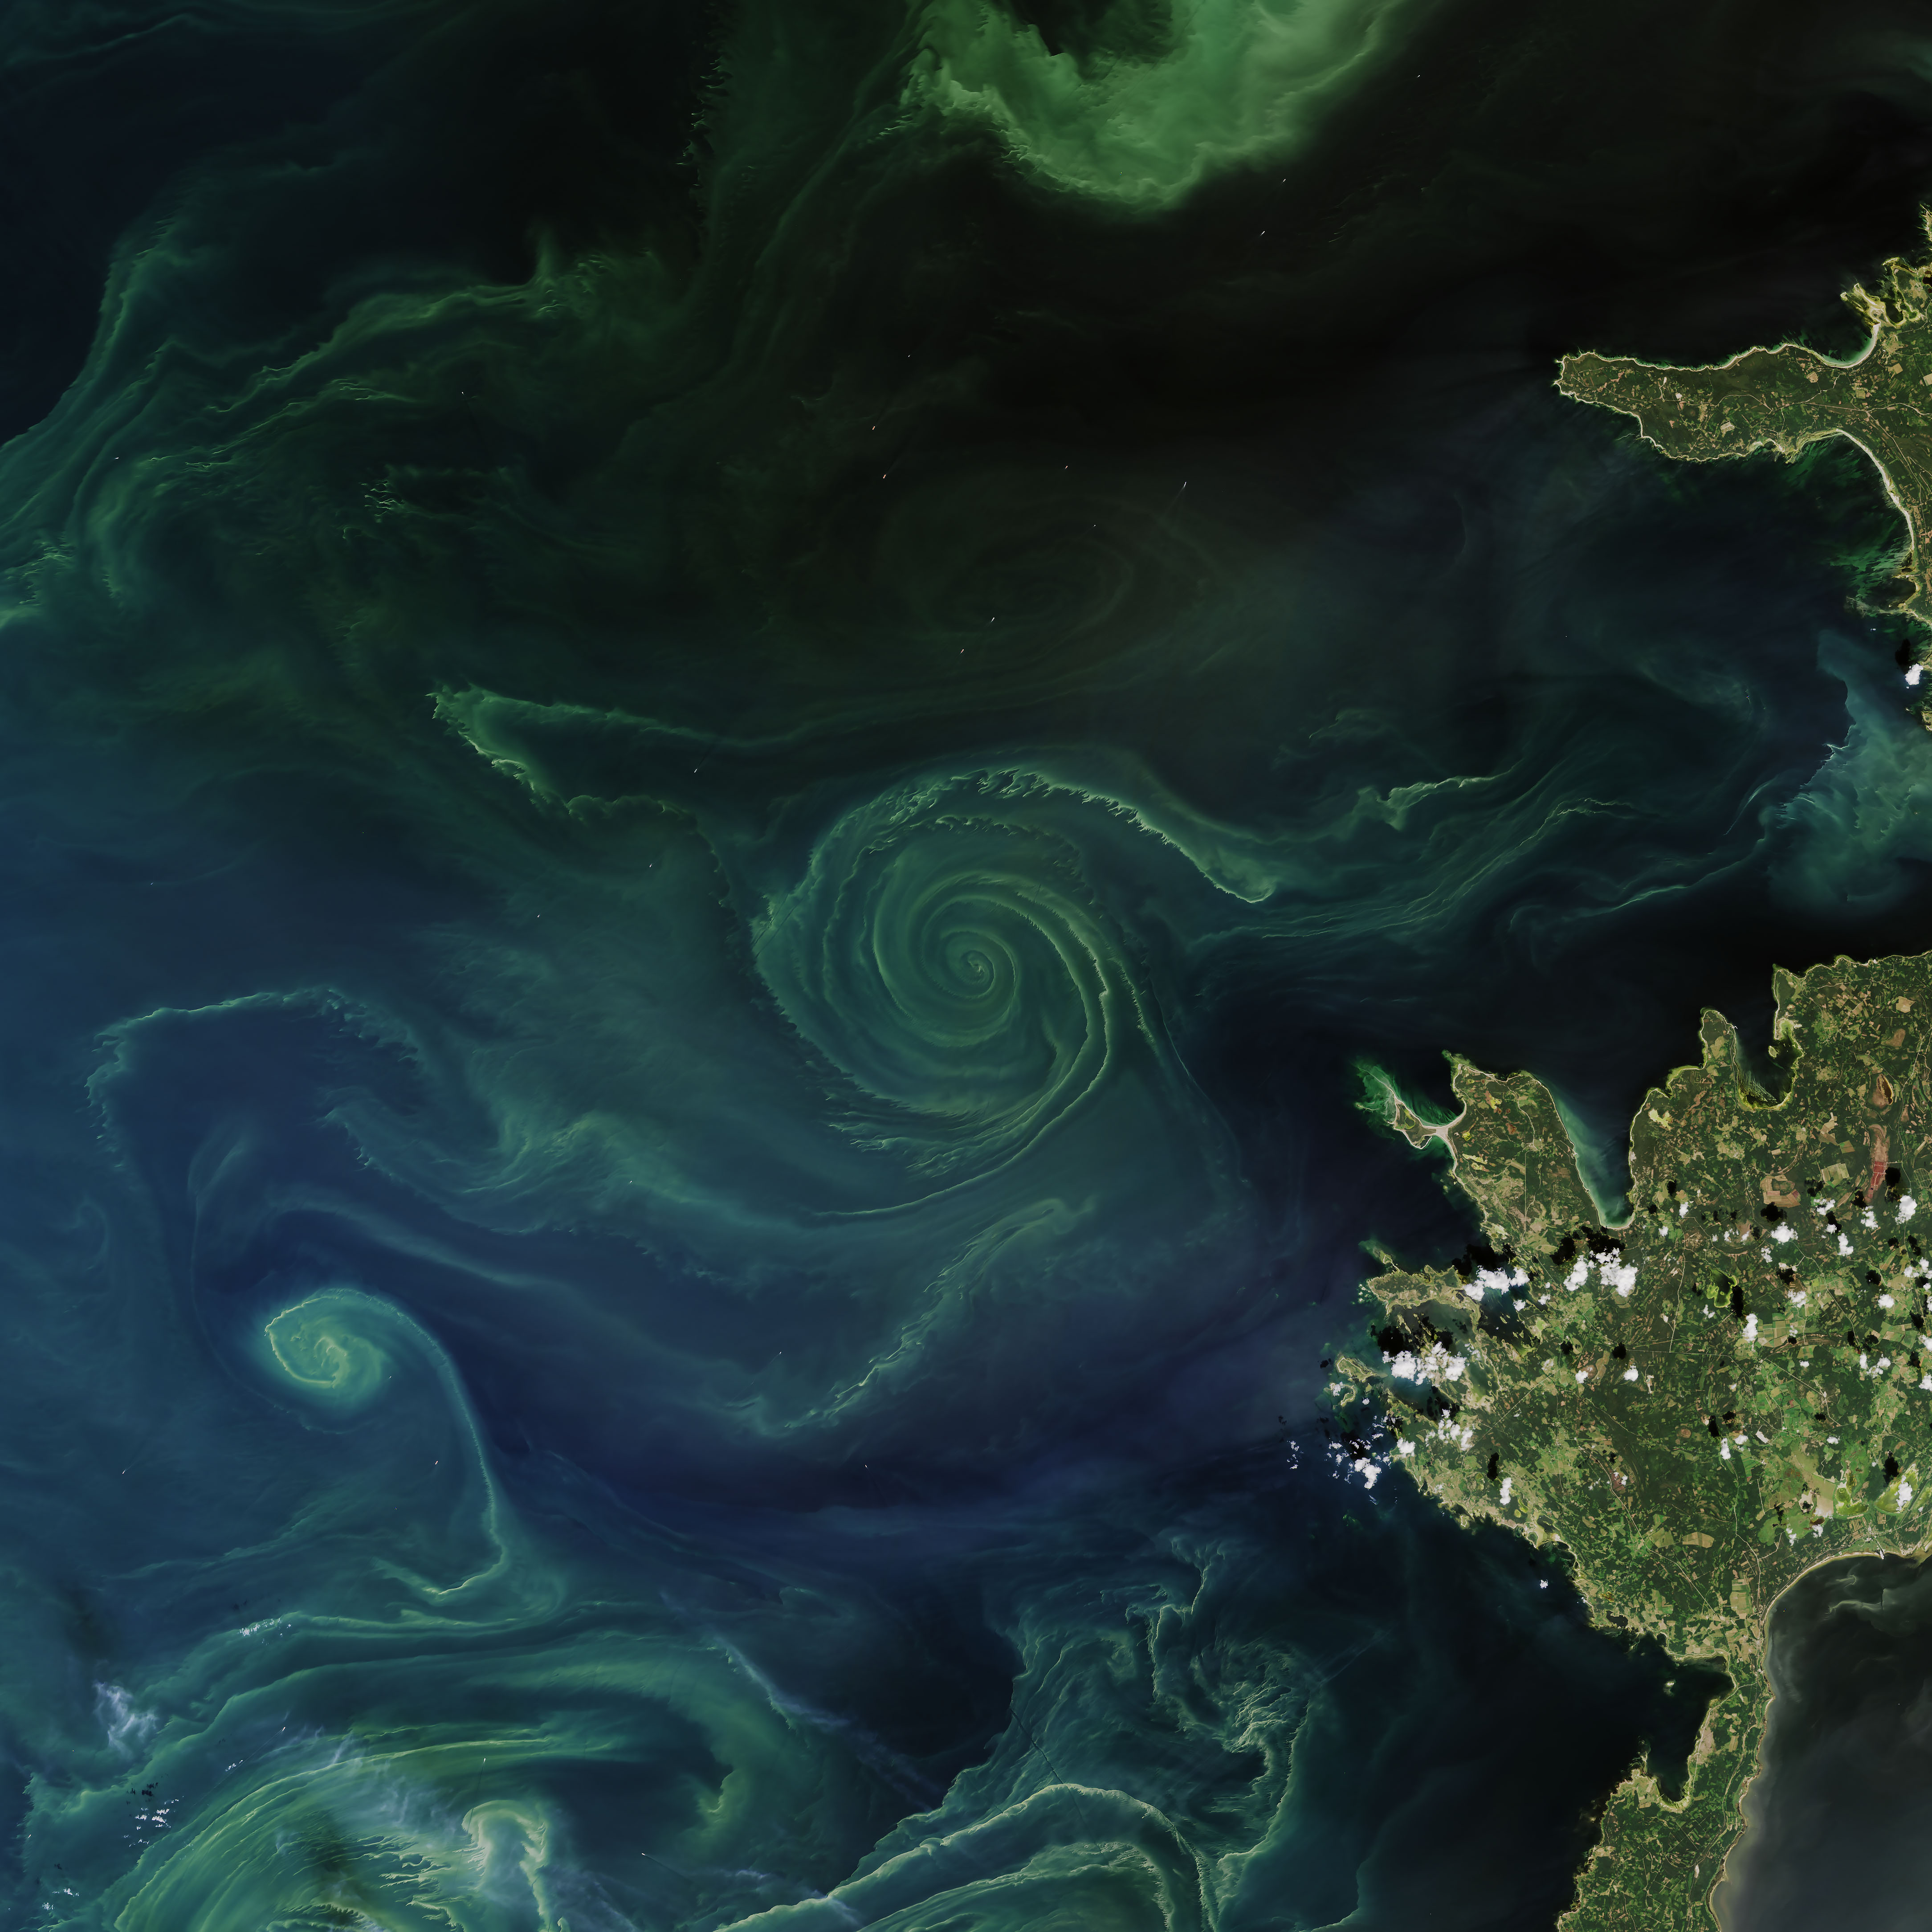
\includegraphics[height=\textwidth]{img/gulfoffinland_oli_2018199_lrg.jpg}
        \caption{}
        \label{fig:sat_finland}
    \end{subfigure}
    \caption{Two satellite images of blooms with different colours, related to the phytoplankton species: in \autoref{fig:sat_barent} the white colour is related to the presence of coccolitophores; in \autoref{fig:sat_finland} there are green cyanobacteria (and possibly diatoms). True colours, source: \url{https://earthobservatory.nasa.gov/images/92462/summer-blooms-in-the-baltic-and-barents}}
    \label{fig:sat_colour}
\end{figure}

\begin{figure} [H]
    \centering
    \begin{subfigure}[b]{\textwidth}
        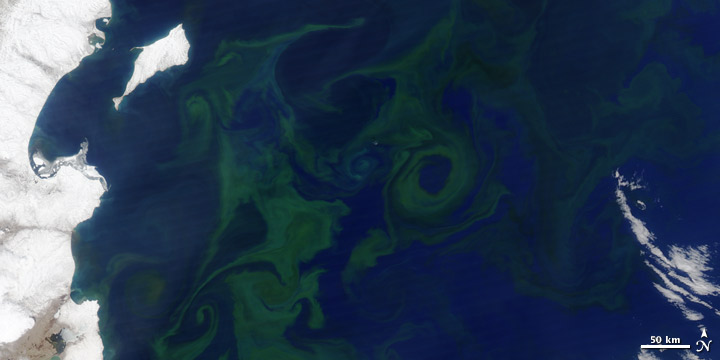
\includegraphics[width=\textwidth]{img/kamchatka_amo_2010153_color.jpg}
        \caption{}
        \label{fig:sat_kamchatka_col}
    \end{subfigure}
    \begin{subfigure}[b]{\textwidth}
        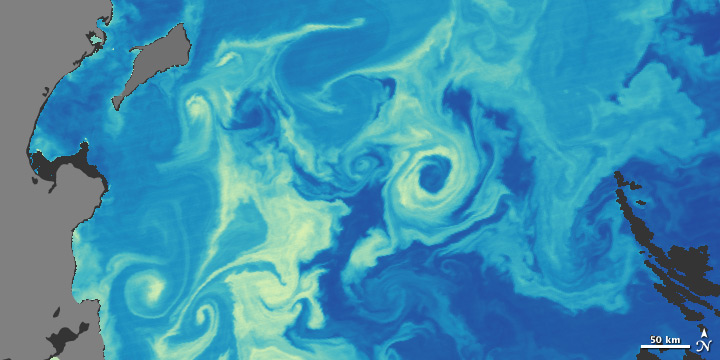
\includegraphics[width=\textwidth]{img/kamchatka_amo_2010153_chlorophyll.jpg}
        \caption{}
        \label{fig:sat_kamchatka_clo}
    \end{subfigure}
    \caption{The same satellite images in true colours (\autoref{fig:sat_kamchatka_col}) and showing the chlorophyll concentration (\autoref{fig:sat_kamchatka_clo}; the palette ranges from blue, $5\cdot 10^{-2}mg/m^3$, to white, $50mg/m^3$). Source: \url{https://earthobservatory.nasa.gov/features/Phytoplankton/page2.php}}
    \label{fig:sat_kamchatka}
\end{figure}

\subsubsection{Distribution} \label{sec:distribution}
The parameters which influence the shape and location of phytoplankton are many: the most important is the fluid flow, which transports cells. The study of this phenomenon is complex, since the flow is turbulent, and the tools of chaotic systems are used to study the Lagrangian flow of particles (see for example \autocite{hernandez2010chemical}). Not only the passive transport of cells is important: the weight and shape of particles \autocite{Toschi2009LagrangianTurbulence}, the growth rate (as this work shows), and the swimming capabilities (both chemotactic \autocite{Taylor2012Trade-offsWater} and gyrotactic \autocite{DeLillo2014TurbulentMicroorganisms,Durham2013TurbulencePhytoplankton}) cause deviations from the bare flow transportation.
Determining the concentration of phytoplankton in a given volume of water is of course difficult, and the direct measurement involves collecting water at different depths and counting the cells \autocite{Sverdrup1953OnPhytoplankton}. Satellite images result useful to address this problem, allowing the identification of blooming areas observing both real colours and chlorophyll characteristic wavelengths. In \autocite{Behrenfeld2010AbandoningBlooms} an example of data analysis based upon satellitar images is described in detail: starting from the measurements of the surface chlorophyll concentration ($Chl_{sat}$) and phytoplankton carbon concentration ($C_{phyt}$, both in $mg\cdot m^{-3}$), it is possible to estimate the phytoplankton biomass (or at least its variations). It is indeed important to remark that, while $Chl_{sat}$ is a highly uncertain quantity, showing big differences when referring to different sources of data, its variations patterns are comparable. Talking about $C_{phyt}$, its estimate is spoiled by the presence of other similar light-scattering sources, but it has been proved to effectively track phytoplankton biomass (\autocite{Behrenfeld2005Carbon-basedSpace}). 

Looking at \autoref{fig:behrenfeld2010alldata}, the main quantities relevant to determine plankton large-scale dynamics are shown. The strong correlation between $Chl_{sat}$ and $C_{phyt}$ is evident. The relations existing between phytoplankton biomass, Mixed Layer Depth (MLD; the depth of the upper, well-mixed layer of the water column) and Photosynthetically Active Radiation (PAR; the radiation comprised in the wavelength interval of 400-700nm) will be discussed in \autoref{sec:previous}.

\begin{figure} [H]
    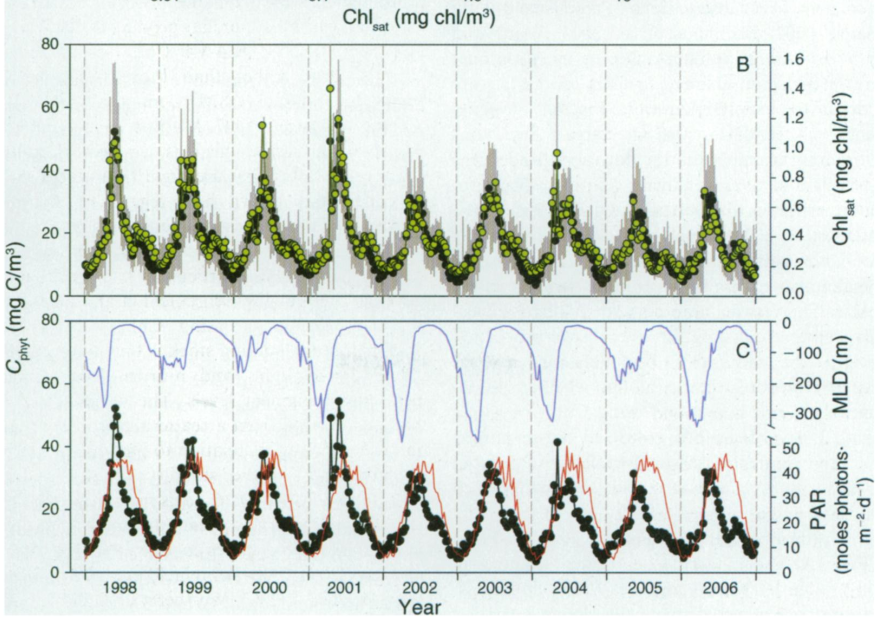
\includegraphics[width=\textwidth]{img/references/behrenfeld2010alldata}
    \caption{This data visualization, taken from \autocite{Behrenfeld2010AbandoningBlooms}, shows $C_{phyt}$ (black dots in both graphs), $Chl_{sat}$ (green dots), MLD (blue line), PAR (red line), over a period of nine years.}
    \label{fig:behrenfeld2010alldata}
\end{figure}

\subsection{Limiting factors}
The present thesis focuses on the dynamics of a population of plankton, ultimately considering the factors which influence the ``birth'' of a new cell or the ``death'' of an existing one. These are well-known from the biological research, and consist in a mix of physical and ecological aspects. One or more of these factors can be \textit{limiting}, meaning that they assume values which limit the population growth. \\
A brief description of the biological and physical processes which influence the dynamics of a phytoplankton population is given below; it will turn out that, during the onset of a bloom, which is here considered, only two factors are necessary: one accounting for the biology, the other for the physics.

In order to reproduce, phytoplankton needs nutrients of different kinds, which are absorbed from water with a combination of passive (diffusive) and active (transport across membranes) mechanisms \autocite[section 4.2]{reynolds2006ecology}; motion can also be an important factor for nutrient uptake when the cell is able to generate large enough turbulence (\( Re>10^{-3}\))\autocite{riebesell2002supply}. The main nutrients needed by phytoplankton are carbon (C), nitrogen (N), phosphorus (P) and iron (Fe): carbon is the most important and the ratio of uptake is approximately \(106 C : 16 N : 1 P : 0.0075 Fe\) \autocite{Bristow2017NutrientsOcean}; these are transported by currents and convective fluxes. \\
% FONTE
The most evident cause of loss for phytoplankton is trophic: as said above, species from very different taxonomic groups are both planktonic and feeding on phytoplankton (a behaviour often referred to as being ``herbivore'', or a ``grazer''). A detailed list can be found in \autocite[chapter 6.4]{reynolds2006ecology}, where a distinction is made between \textit{filter-feeding}, that is the feeding strategy of filtering out of the ingested water any big enough particles, and \textit{selective feeding}. When the former strategy is favorable, it has a bigger impact on the phytoplankton population, potentially wiping it off. As pointed out by Taylor in \autocite{Taylor2011ShutdownBlooms}, the relatively short amount of time characterizing the onset of a bloom (order of weeks) allows to assume that the ``herbivorous'' population does not have the time to grow at the same pace; this means that the loss rate due to grazing can be modeled with a constant loss rate coefficient. \\
Another harm for phytoplankton population are pathogens: fungi, protozoans, viruses and bacteria are part of this category\autocite[section 6.5]{reynolds2006ecology}. The models here considered include their effect by tuning the loss rate coefficient. 

The factors physically influencing phytoplankton reproduction are connected to the availability of light experienced by the cells: this can be influenced by the turbidity of water, and by how the water flow and the sink move the cells with respect to this scalar field. The viscous drag experienced by a spherical cell is given by Stokes' law:
\[f = 6 \pi \eta a\]
where $a$ is the radius of the cell and $\eta$ is the viscosity \autocite[chapter 4]{berg1993random}.

\subsection{Ecological importance}
Phytoplankton is accounted to be responsible for half of the oxygen produced on the planet (although some estimates indicate an even bigger percentage), as well as half of the biosphere \textit{Net Primary Production}\footnote{The Net Primary Production (NPP) is a measure of the production of organic compounds, from which is subtracted the part that is instead consumed.}\autocite{Behrenfeld2006Climate-drivenProductivity}. In \autocite{Sekerci2015MathematicalChange} a mathematical model, suggesting that global warming could cause the depletion of oxygen from atmosphere and highlighting one more time the importance of phytoplankton in the planetary ecosystem. Organic matter produced by phytoplankton in the upper ocean partly is consumed by grazers, partly sinks reaching the bottom of the ocean, possibly sedimenting and going through the process which transforms it in oil \autocite{Falkowski2012OceanPlankton}. 
